\let\negmedspace\undefined
\let\negthickspace\undefined
\documentclass[journal]{IEEEtran}
\usepackage[a5paper, margin=10mm, onecolumn]{geometry}
%\usepackage{lmodern} % Ensure lmodern is loaded for pdflatex
\usepackage{tfrupee} % Include tfrupee package

\setlength{\headheight}{1cm} % Set the height of the header box
\setlength{\headsep}{0mm}     % Set the distance between the header box and the top of the text
\usepackage{gvv-book}
\usepackage{gvv}
\usepackage{cite}
\usepackage{amsmath,amssymb,amsfonts,amsthm}
\usepackage{algorithmic}
\usepackage{graphicx}
\usepackage{textcomp}
\usepackage{xcolor}
\usepackage{txfonts}
\usepackage{listings}
\usepackage{enumitem}
\usepackage{mathtools}
\usepackage{gensymb}
\usepackage{comment}
\usepackage[breaklinks=true]{hyperref}
\usepackage{tkz-euclide} 
\usepackage{listings}
% \usepackage{gvv}                                        
\def\inputGnumericTable{}                                 
\usepackage[latin1]{inputenc}                                
\usepackage{color}                                            
\usepackage{array}                                            
\usepackage{longtable}                                       
\usepackage{calc}                                             
\usepackage{multirow}                                         
\usepackage{hhline}                                           
\usepackage{ifthen}                                           
\usepackage{lscape}
\begin{document}

\bibliographystyle{IEEEtran}
\vspace{3cm}

\title{8.3.13}
\author{EE24BTECH11027 - satwikagv}
% \maketitle
% \newpage
% \bigskip
{\let\newpage\relax\maketitle}

\renewcommand{\thefigure}{\theenumi}
\renewcommand{\thetable}{\theenumi}
\setlength{\intextsep}{10pt} % Space between text and floats


\numberwithin{equation}{enumi}
\numberwithin{figure}{enumi}
\renewcommand{\thetable}{\theenumi}
\textbf{Question}:
Find the area of the triangle $ABC$  whose vertices have the coordinates $A\brak{2,0}$ ,$B\brak{4,5}$ and $C\brak{6,3}$\\
\textbf{Solution}:\\
\textbf{Numerical method}:\\
\begin{center}
\begin{tikzpicture}[scale=0.9,rotate=-38]
\coordinate (A) at (2,0);
\coordinate (B) at (4,5);
\coordinate (C) at (6,3);

\draw[thick, black] (B) -- (C) -- (A) node[midway,below]{$b$} -- cycle;
\node[below left] at (A) {$A(2, 0)$};
\node[above] at (B) {$B(4, 5)$};
\node[below right] at (C) {$C(6, 3)$};
\draw[thick,black] (B) -- (5.68,2.76) node[midway,left] {$h$};
\filldraw[black] (A) circle (2pt);
\filldraw[black] (B) circle (2pt);
\filldraw[black] (C) circle (2pt);

\end{tikzpicture}
\end{center}
Here $b$,$h$ are the base, height of the triangle.\\
The base $b$ of the triangle is the distance between the points $A$ and $C$ and is calculated as 
\begin{align}
    b=\sqrt{\brak{6-2}^2+\brak{3-0}^2}\\
    b=5
\end{align}
The height $h$ of the triangle is the perpendicular distance from the point $B$ to the line $AC$
The eq of the line passing through $A$,$C$ is calculated as 
\begin{align}
    3x-4y-6=0
\end{align}
The height of the triangle is calculated as 
\begin{align}
    h=\frac{\abs{3\brak{4}-4\brak{5}-6}}{\sqrt{3^2+4^2}}\\
    h=\frac{14}{5}
\end{align}
The area of the triangle $ABC$ is 
\begin{align}
    \text{area}=\frac{1}{2}bh\\
    \text{area}=\frac{1}{2}\times5\times\frac{14}{5}\\
    \text{area}=7 \text{sq.units}
\end{align}
Therefore, the area of the triangle formed by points $A$,$B$ and $C$ is 7 sq.units\\\\
\textbf{Trapezoidal rule}:\\
Trapezoidal rule is the approximation of the definite integral of a function by dividing the area under the curve into trapezoids and summing up the areas.\\The area of a trapezoid $A_T$ is given as 
\begin{align}
    A_T=\frac{h}{2}\brak{a+b}
\end{align}
where $h$ is the height of the trapezoid and $a$,$b$ are the lengths of the parallel sides of the trapezoid. \\
To find the area under the function $y\brak{x}$ over a interval \sbrak{a,b} is the sum of the area of the $n$ trapezoids of equal width divided in between them.\\
Let $a=x_0,b=x_n$ and $A_k$ be the area under the curve $y\brak{x}$ from $x=x_0$ to $x=x_k$.And we  can define the following relation
\begin{align}
    A_{k+1}=A_k+\frac{h}{2}\brak{y_k+y_{k+1}}
\end{align}
where,
\begin{align}
    y_{k+1}=y_k+hy^\prime_k\\
    x_{k+1}=x_k+h
\end{align}
Here $h=\frac{b-a}{n}$
Substitute eq \brak{0.11} in eq \brak{0.10},we get
\begin{align}
    A_{k+1}=A_k+\frac{h}{2}\brak{2y_k+hy^\prime_k}\\
    A_{k+1}=A_k+hy_k+\frac{h^2}{2}\brak{y^\prime_k}
\end{align}
The sum of the areas of the trapezoids from $k=0$ to $k=n-1$ we get the approximated area $A$, under the curve as
\begin{align}
A=\int_a^by\brak{x}=\frac{h}{2}\brak{y\brak{x_0}+2y\brak{x_1}+2y\brak{x_2}+\dots+y\brak{x_n}}
\end{align}
So, from the above rule the area of the triangle can be computed as:
\\Let say now $a$ be the area of the triangle $ABC$ we need to calculated and it can be as:
\begin{align}
a=\text{Area under } AB + \text{Area under }BC - \text{Area under }AC
\end{align}
SO, the line equations of the lines are being calculated as:
\begin{align}
    AB:y=\frac{5}{2}x-5 \text{ and } y^\prime=\frac{5}{2}\\BC:y=-x+9\text{ and } y^\prime=-1\\AC:y=\frac{3}{4}x-\frac{3}{2} \text{ and }y^\prime=\frac{3}{4}
\end{align}
For the line $AB$ the area equation is written as:
\begin{align}
    A_{k+1}=A_k+h\brak{\frac{5}{2}x_k-5}+\frac{h^2}{2}\brak{\frac{5}{2}}
\end{align}
Taking $x_0=2$ to $x_n=4$
\begin{align}
    \text{area under }AB=A_n=5
\end{align}
For the line $BC$ the area equation is written as:
\begin{align}
    A_{k+1}=A_k+h\brak{-x_k+9}+\frac{h^2}{2}\brak{-1}
\end{align}
Taking $x_0=4$ and $x_n=6$
\begin{align}
    \text{area under }BC=A_n=8
\end{align}
For the line $AC$ the area equation is written as:
\begin{align}
    A_{k+1}=A_k+h\brak{\frac{3}{4}x_k-\frac{3}{2}}+\frac{h^2}{2}\brak{\frac{3}{4}}
\end{align}
Taking $x_0=2$ and $x_n=6$
\begin{align}
    \text{area under }CA=6
\end{align}
Therefore, the area of the triangle is,\\from eq \brak{0.16} is
\begin{align}
    a=5+8-6\\a=7
\end{align}
Clearly, from eq\brak{0.8} and eq\brak{0.27}, the area of the triangle in both methods is same.
\textbf{Plotting the triangle using difference equation}:\\
To plot the triangle using difference equations we can use the equations \brak{0.11} and \brak{0.12}\\For the line AB,from eq\brak{0.17} we have
\begin{align}
    y_{k+1}=y_k+\frac{5}{2}h
\end{align}
For the line $BC$, from eq\brak{0.18} we have
\begin{align}
    y_{k+1}=y_k-h
\end{align}
For the line $AC$, from eq\brak{0.19} we have
\begin{align}
    y_{k+1}=y_k+\frac{3}{4}h
\end{align}
For more accuracy the $h$ should be small and iteratively run the above three equations to get the triangle plot.\\The curve generated using method of differences is compared with the actual plot of the triangle in the figure below.
\begin{figure}[h!]
   \centering
   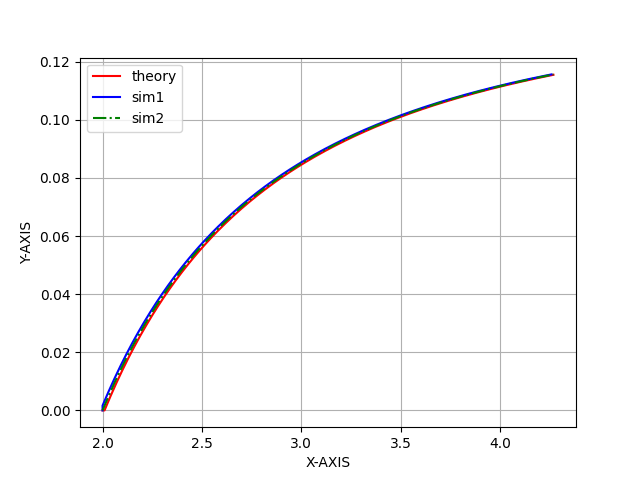
\includegraphics[width=\columnwidth]{figs/fig.png}
\end{figure}
\end{document}
